%
% 計測自動制御学会システム・情報部門学術講演会2013原稿サンプルファイル
%                                           August 26, 2013
% 計測自動制御学会システム・情報部門学術講演会2011原稿サンプルファイル
%                                           April 28, 2011
% Based on 第7回計測自動制御学会制御部門大会原稿サンプルファイル
%                                           October 18, 2007
% Based on 第5回計測自動制御学会制御部門大会原稿サンプルファイル
%            近野敦 konno@space.mech.tohoku.ac.jp    March 05, 2005
%
% LaTeX2eとLaTeX209判別のための定義(以下3行)は科研費マクロkkhgrp.mac
% の定義を,作者の金沢大学青木先生の許可を得て利用させていただきました.
%
\newif\ifLaTeXe\LaTeXefalse
\expandafter\ifx\csname PackageError\endcsname\relax\LaTeXefalse
\else\LaTeXetrue\fi

\ifLaTeXe
  \documentclass{jarticle}
  \usepackage{SICE-SSI}
 % \usepackage[dvips]{graphicx}
  \usepackage[dvipdfmx]{graphicx}
\else
  \documentstyle[SICE-SSI,epsbox]{jarticle}
\fi

\begin{document}
\title{UPPAALによる交差点における自動運転車群のモデル化と検証}
\author{○佐原優衣\ 中村正樹\ 榊原一紀\ (富山県立大学)\ 玉置久\ (神戸大学)}

\abstract{
  本研究では自動運転車群による交差点通過の制御アルゴリズムを,UPPAALツールにより時間オートマトンとして形式的にモデル化し,モデル検査技術を用いて,追従も含めたアルゴリズムで,最小時間を検証する手法を検討する.
  }

\keyword{自動運転車制御,形式検証,時間オートマトン,UPPAAL}

\maketitle\thispagestyle{empty}
\pagestyle{empty}

\section{はじめに}
近年,自動運転技術が急速に発達している. 自動運転は,搭載される技術によってレベル1からレベル5までに分けられており,現在,日本国内では,運転者支援を主としたレベル2までが市販車に採用されている.今後,高速道路や,限定地域での特定条件下での完全自動運転を行うレベル4の車両の普及が目指されている.
自動運転技術が普及し,大量の自動運転車が利用される都市空間を考える.
道路上の車両密度が高くなるため,渋滞やデッドロックが発生することが想定される.したがって,個々の車両だけではなく,自動運転車群が効率的に走行するアルゴリズムが必要となる.

本研究では群制御アルゴリズムが安全性に関わる衝突回避やデッドロック回避,効率性に関わる時間制約などの性質を満たすかどうかを検証する手法を提案する.
自動運転車の群制御アルゴリズムを形式的に記述し,モデル検査を用いて,性質を検証する.モデル検査は,システム上で起こり得る状態を網羅的に調べることにより設計の誤りを発見する自動検証手法の一種である.モデル検査手法は,システムの振る舞いの設計,および検証したい性質をそれぞれモデル化し,ツールを用いて,システムが性質を満たしているかを調べる.
本研究では,時間オートマトン\cite{u3}による時間制約検証が行えるモデル検査ツールUPPAAL\cite{u1,u2}を採用する.
UPPAALを用いて交差点を通過する1台の自動運転車の挙動をモデル化する。交差点は2車線対面通行で右折用レーンはなく,信号もない交差点とする.
\section{追従のない交差点モデル}
本節では先行研究\cite{a,a1}で扱った同一方向の追従のない交差点を用いて,UPPAALによる交差点のモデル化,シミュレーション,検証の方法を紹介する
車両は自分の始点と終点を保持し,挙動を交差点進入前,交差点通過中,交差点通過後の3つの状態に分類する.交差点には5つの鍵があるとして,その組み合わせで交差点の使用権を管理するモデルを考えた.交差点通過には,同時に通行可能な組み合わせと,そうでない組み合わせがある.例えば,対面の直進同士は同時通行可能だが,対面の直進と右折は同時通行不可である.交差点内に5つの地点を設定し,各進入方向からの直進右左折が,どの地点を通過するかを分析することで,交差点の使用権を考える.交差点内の5つ地点にそれぞれ鍵を設定し,その組み合わせで交差点を通過可能とする.
\subsection{時間オートマトン}
進行方向と直進右左折を固定した車両の時間オートマトンを作成する.
この時間オートマトンは,パラメータ変数としてL1, L2, useを持ち,
各車両が管理する時間変数local\_clockを持つ.
L1, L2は,インスタンス生成時に,lock1, lock2, lock3, lock4のいずれで具象化される.useにより,地点crossを通過するかどうかを0, 1で表す.
Fig.\ref{Simple}に,時間オートマトンを示す.

	\begin{figure}[htbp]
	\centering
	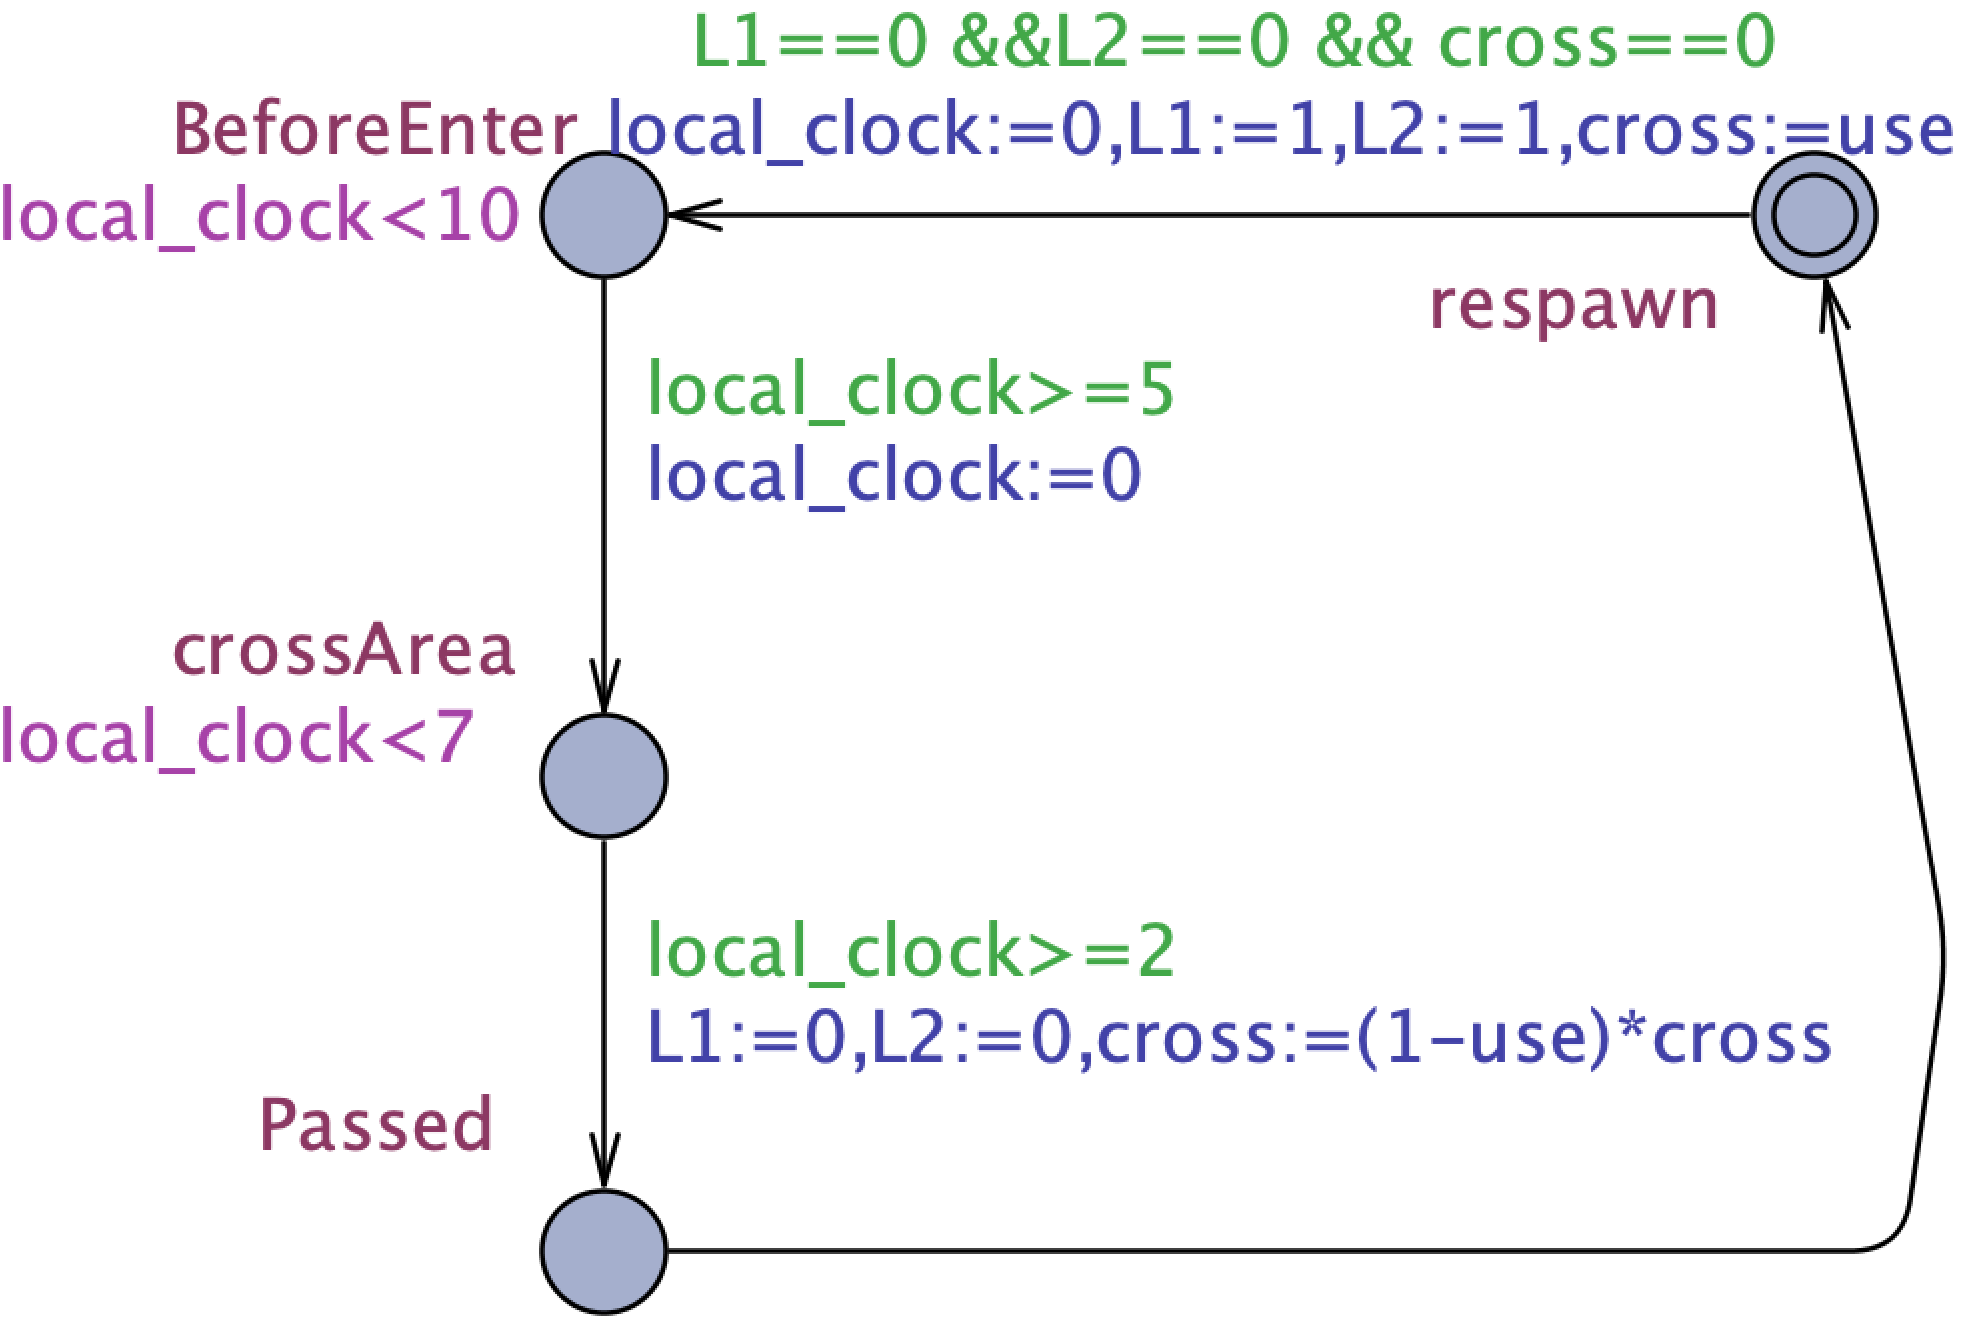
\includegraphics[width=65mm]{SimpleIntersection.png}
	\caption{交差点を通過する車両の時間オートマトン}
	\label{Simple}
	\end{figure}
パラメータL1,L2,右折用鍵crossが取得可能(値が0)なとき,
初期状態respawnから交差点進入前状態BeforeEnterへの遷移可能とする.
遷移時,L1, L2を他の車両から取得できないようにする(1に更新).
crossをuseで更新する.交差点を使用する車両のときのみ,crossが使用中となる.
また,時間変数local\_clockを0に更新する.
BeforeEnter状態には,local\_clockが10秒未満という条件が付与されている.BeforeEnterからの遷移には,5秒以上という条件が付与されている.
直前に時間変数がリセットされているため,これらの条件から,
BeforeEnter状態には5秒以上10秒未満の期間内のみいられることが記述されている.
同様に,crossArea状態には2秒以上7秒未満の時間制約が与えられる.
crossArea状態からPassed状態への遷移時に,
L1, L2の使用権が解放される.
また,crossの更新では,地点crossの仕様の有無に関わらずcrossが0に更新される.
\subsection{シミュレーション}
直進は対応する鍵をL1, L2に設定してる.
左折は,L1, L2に同じ鍵を設定している.
右折は,L1, L2に対応する鍵を与え,useに1を与えている.
Fig.\ref{SimpleS}は,12のインスタンスのうち3台(se, es, wn)が交差点を同時に通過している状態のスクリーンショットである.
	\begin{figure}[htbp]
	\centering
	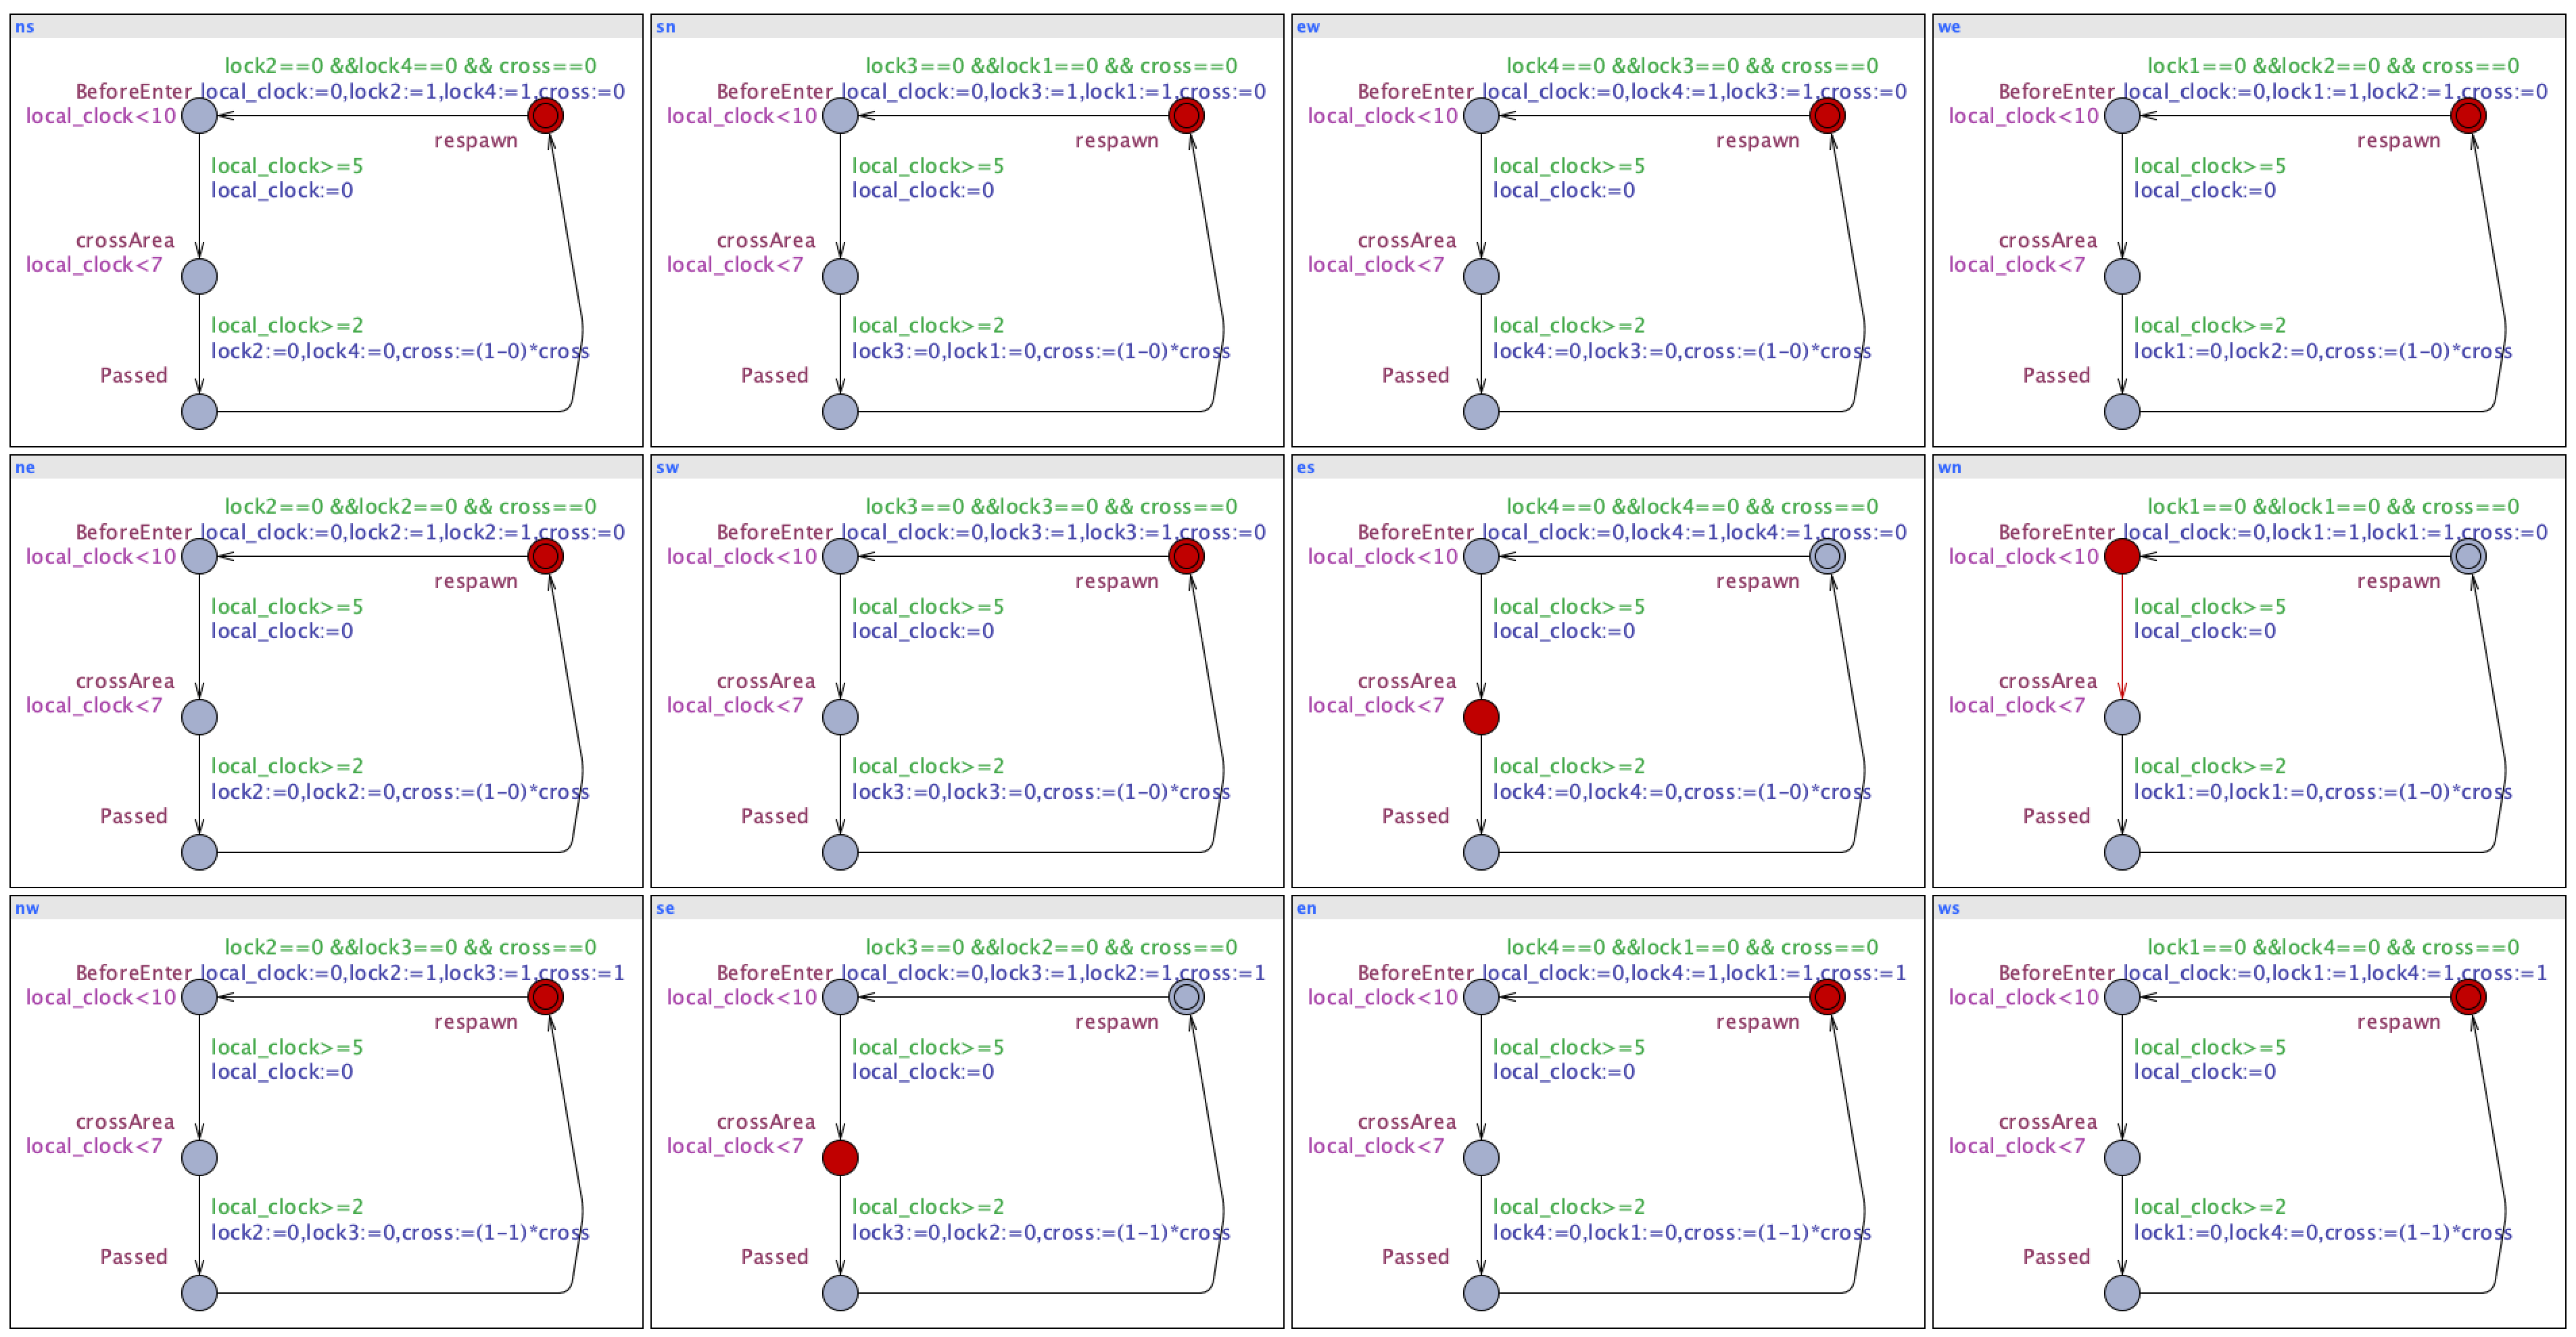
\includegraphics[width=60mm]{SimpleIntersectionSimu.png}
	\caption{交差点を通過する車両の時間オートマトンの合成}
	\label{SimpleS}
	\end{figure}
\subsection{モデル検査}
車両全てが交差点を1回通過するのにかかる最小時間について検証を行う.交差点の使用権の取得方法は前節と同仕様の5つ鍵によって管理する.1回だけなので循環する時間オートマトンではなく一度通過するだけの時間オートマトンを作成する(Fig.\ref{minT}).ループになっていない以外は,Fig.\ref{Simple}と同じである.
最小時間の検証を行う.検証のために大域時間変数gcを宣言する.まず,42秒で全車両が通過できるかどうかを次の検証式を用いて検査する.
	
	\begin{verbatim}
	E<> (gc==42 and ns.finish and sn.finish and 
	... and ws.finish)	
	\end{verbatim}
この検証式は,経過時間が42秒のときに,nsからwsまでのすべての時間オートマトンが状態finishとなる実行列が存在することを表している.
UPPAALモデル検査により,上記の検証式が満たされることが確かめられた.
次に,以下の検証式を考える.
	\begin{verbatim}
	A[] (gc<42 imply not (ns.finish and sn.finish  
	and ... and ws.finish))
	\end{verbatim}
この検証式は,すべての実行列で,経過時間が42秒未満ならばすべての時間オートマトンが状態finishにならないことを表している.
UPPAALモデル検査により,上記の検証式が満たされることが確かめられた.
	\begin{figure}[htbp]
	\centering
	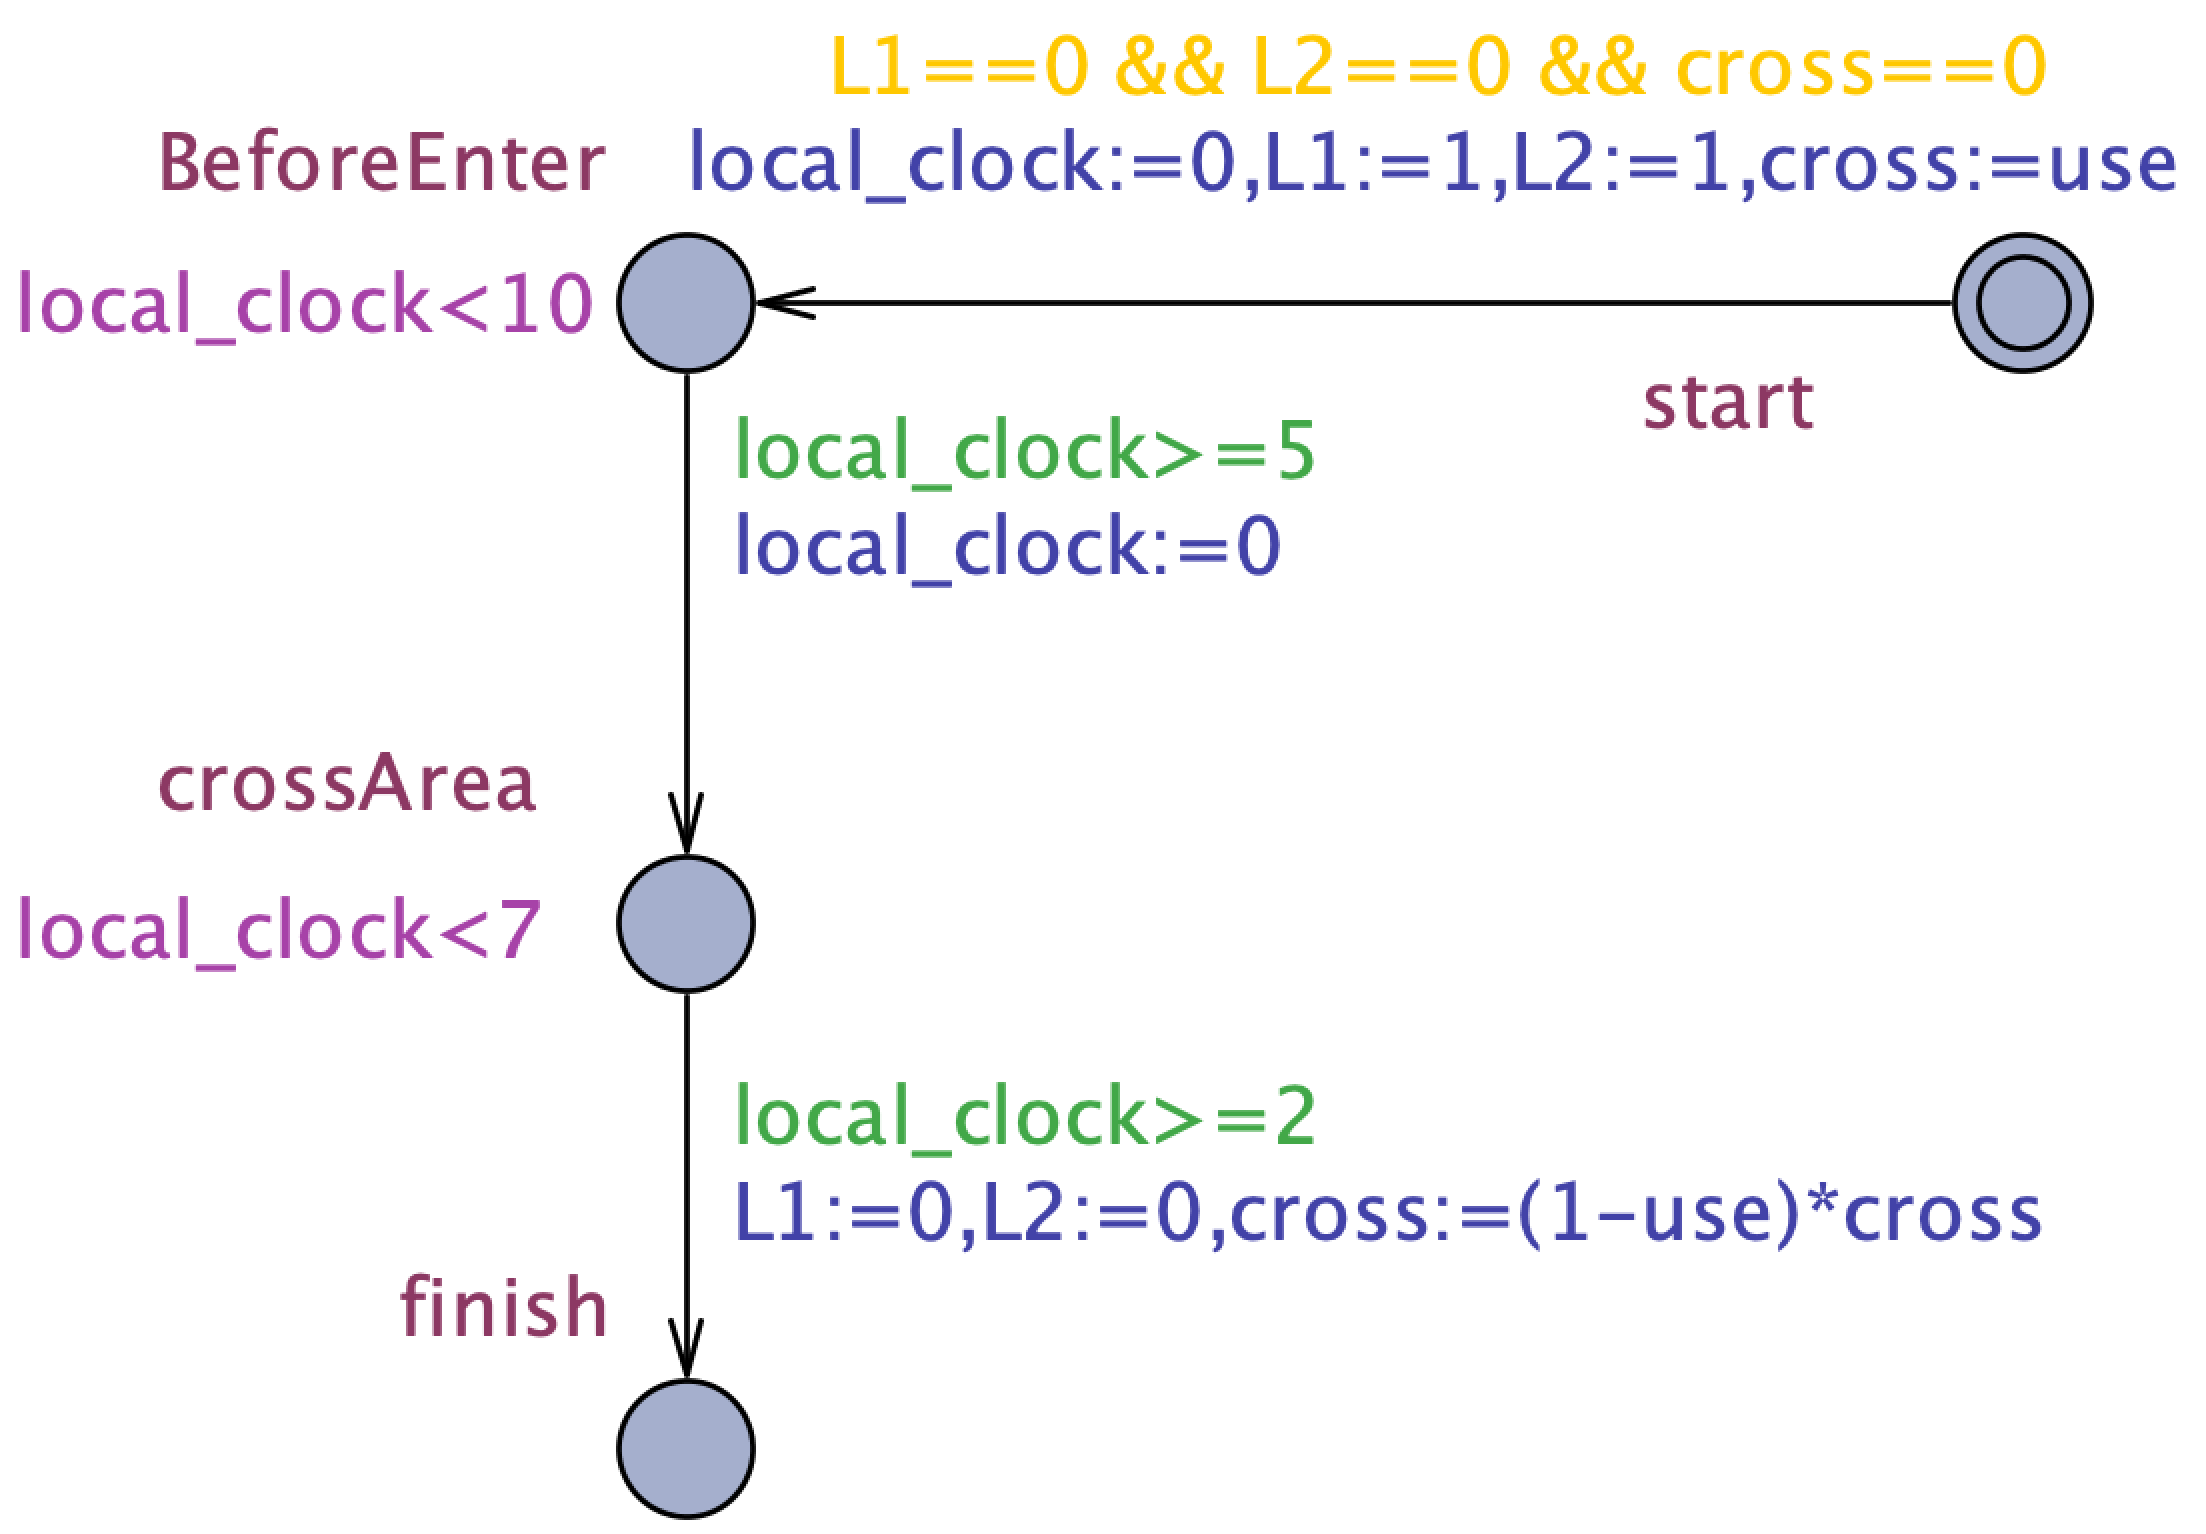
\includegraphics[width=70mm]{minTime.png}
	\caption{交差点を1回通過する時間オートマトン}
	\label{minT}
	\end{figure}
UPPAALモデル検査を用いることで,検証時に具体的な実行列を得ることができる.42秒で通過可能な検証式のモデル検査で,Fig.\ref{veriT}の実行列を得た.
この順番で各車両が交差点を通過することで,42秒で全車両の通過が可能であることが確かめられたことになる.
	
	\begin{figure}[htbp]
	\centering
	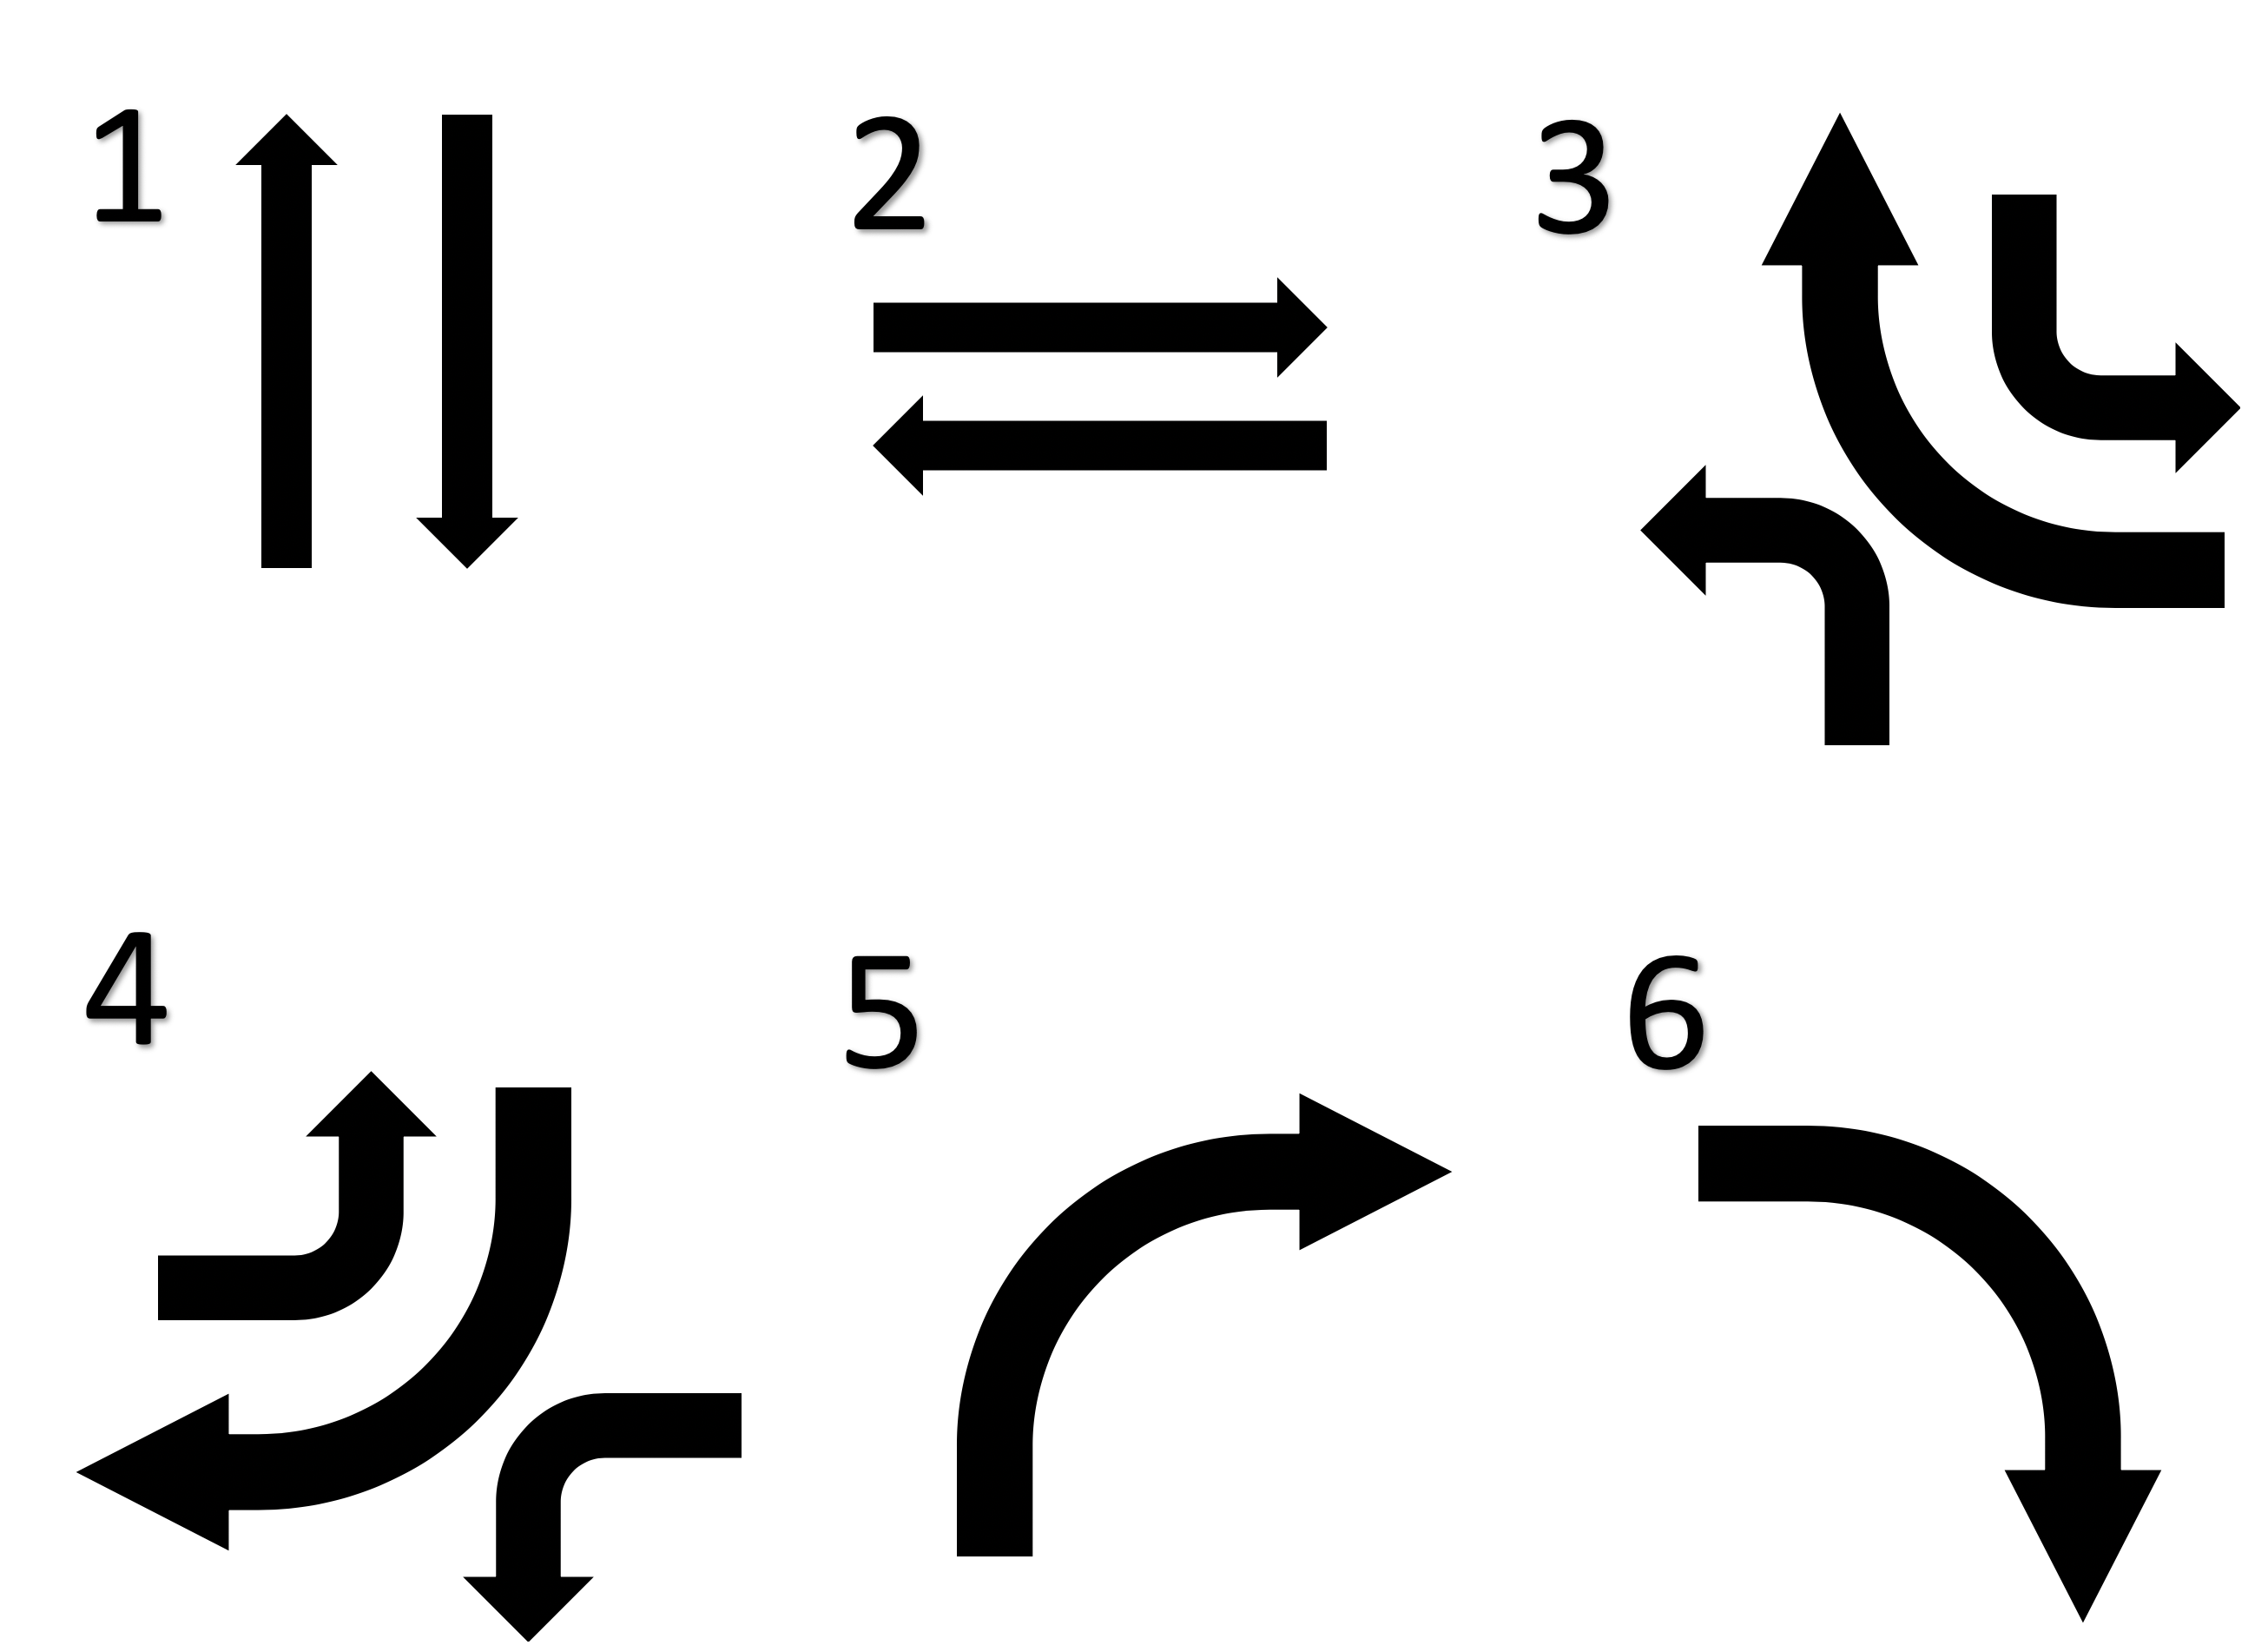
\includegraphics[width=50mm]{veriT.png}
	\caption{最小時間のルート}
	\label{veriT}
	\end{figure}

\section{追従を可能した交差点モデル}
前章のモデルでは,同方向車両が存在した場合,先行した車両が通行終了するまで,後方車両は交差点を通行できなかった.
本章では,例えば同一方向の車両であれば,前方車が時間内に交差点を通過する仮定のもとで,追従して交差点に進入可能なモデルを作成する.
制御器は,交差点通過を2段階に分けて管理し,通過する各車両がどの段階にあるかを把握しているとする.
Fig.\ref{map}の外側の円が交差点通過の第一段階,内側の円が第二段階に対応する.ある車両が北から直進して第二段階で通過中を考える.南から直進または左折する車両は通行可能だが,南から右折する車両は通行できない.一方で西から左折する車両も通行可能である.このとき,北から直進する車両の後続車両が直進や左折の場合,追従可能であるが,右折の場合,追従不可である.
	\begin{figure}[htbp]
	\centering
	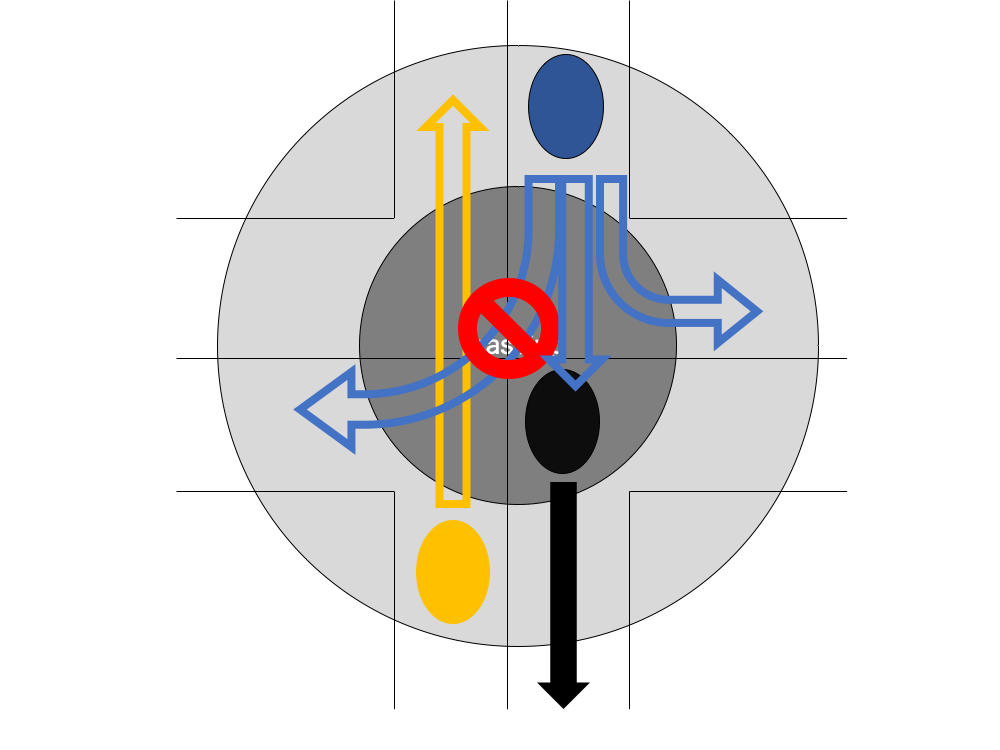
\includegraphics[width=70mm]{model.png}
	\caption{交差点の車両の位置範囲}
	\label{map}
	\end{figure}

\subsection{時間オートマトン}
交差点に対して進入する方向と,直進右左折を保持した車両の時間オートマトンを作成する(Fig.\ref{TAuto}).この時間オートマトンは,パラメータ変数として,交差点に対して進入する方向start,直進右左折を示すturnを持つ.各車両が管理する時間変数timeを持つ.グローバルな二次元配列dir[start][turn]によって,startからturn方向へ通過する車両の総数を管理する.述語go()は,各方向,各段階の現在の車両数から,新たな車両が第一段階に移行かどうかを判定する述語として定義される.
	\begin{figure*}[htbp]
	\centering
	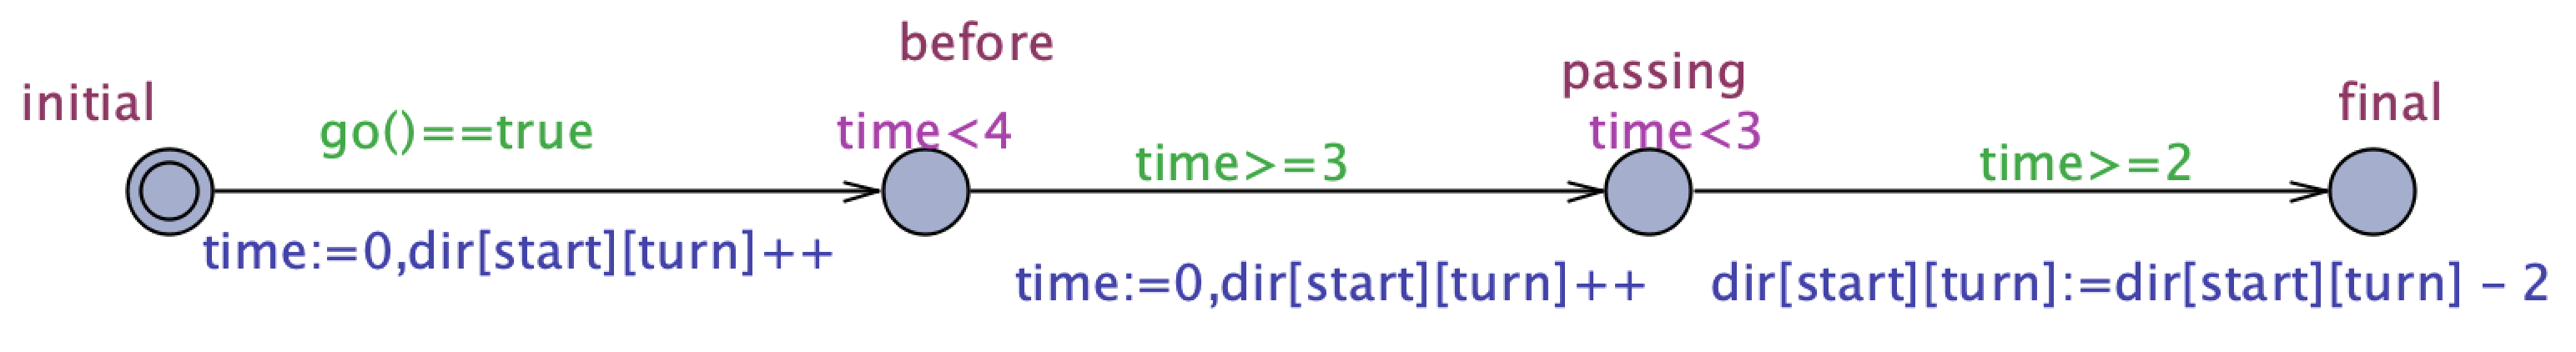
\includegraphics[width=130mm]{TAuto.png}
	\caption{交差点を通過する車両の時間オートマトン}
	\label{TAuto}
	\end{figure*}

\subsection{シミュレーション}
	\begin{figure}[htbp]
	\centering
	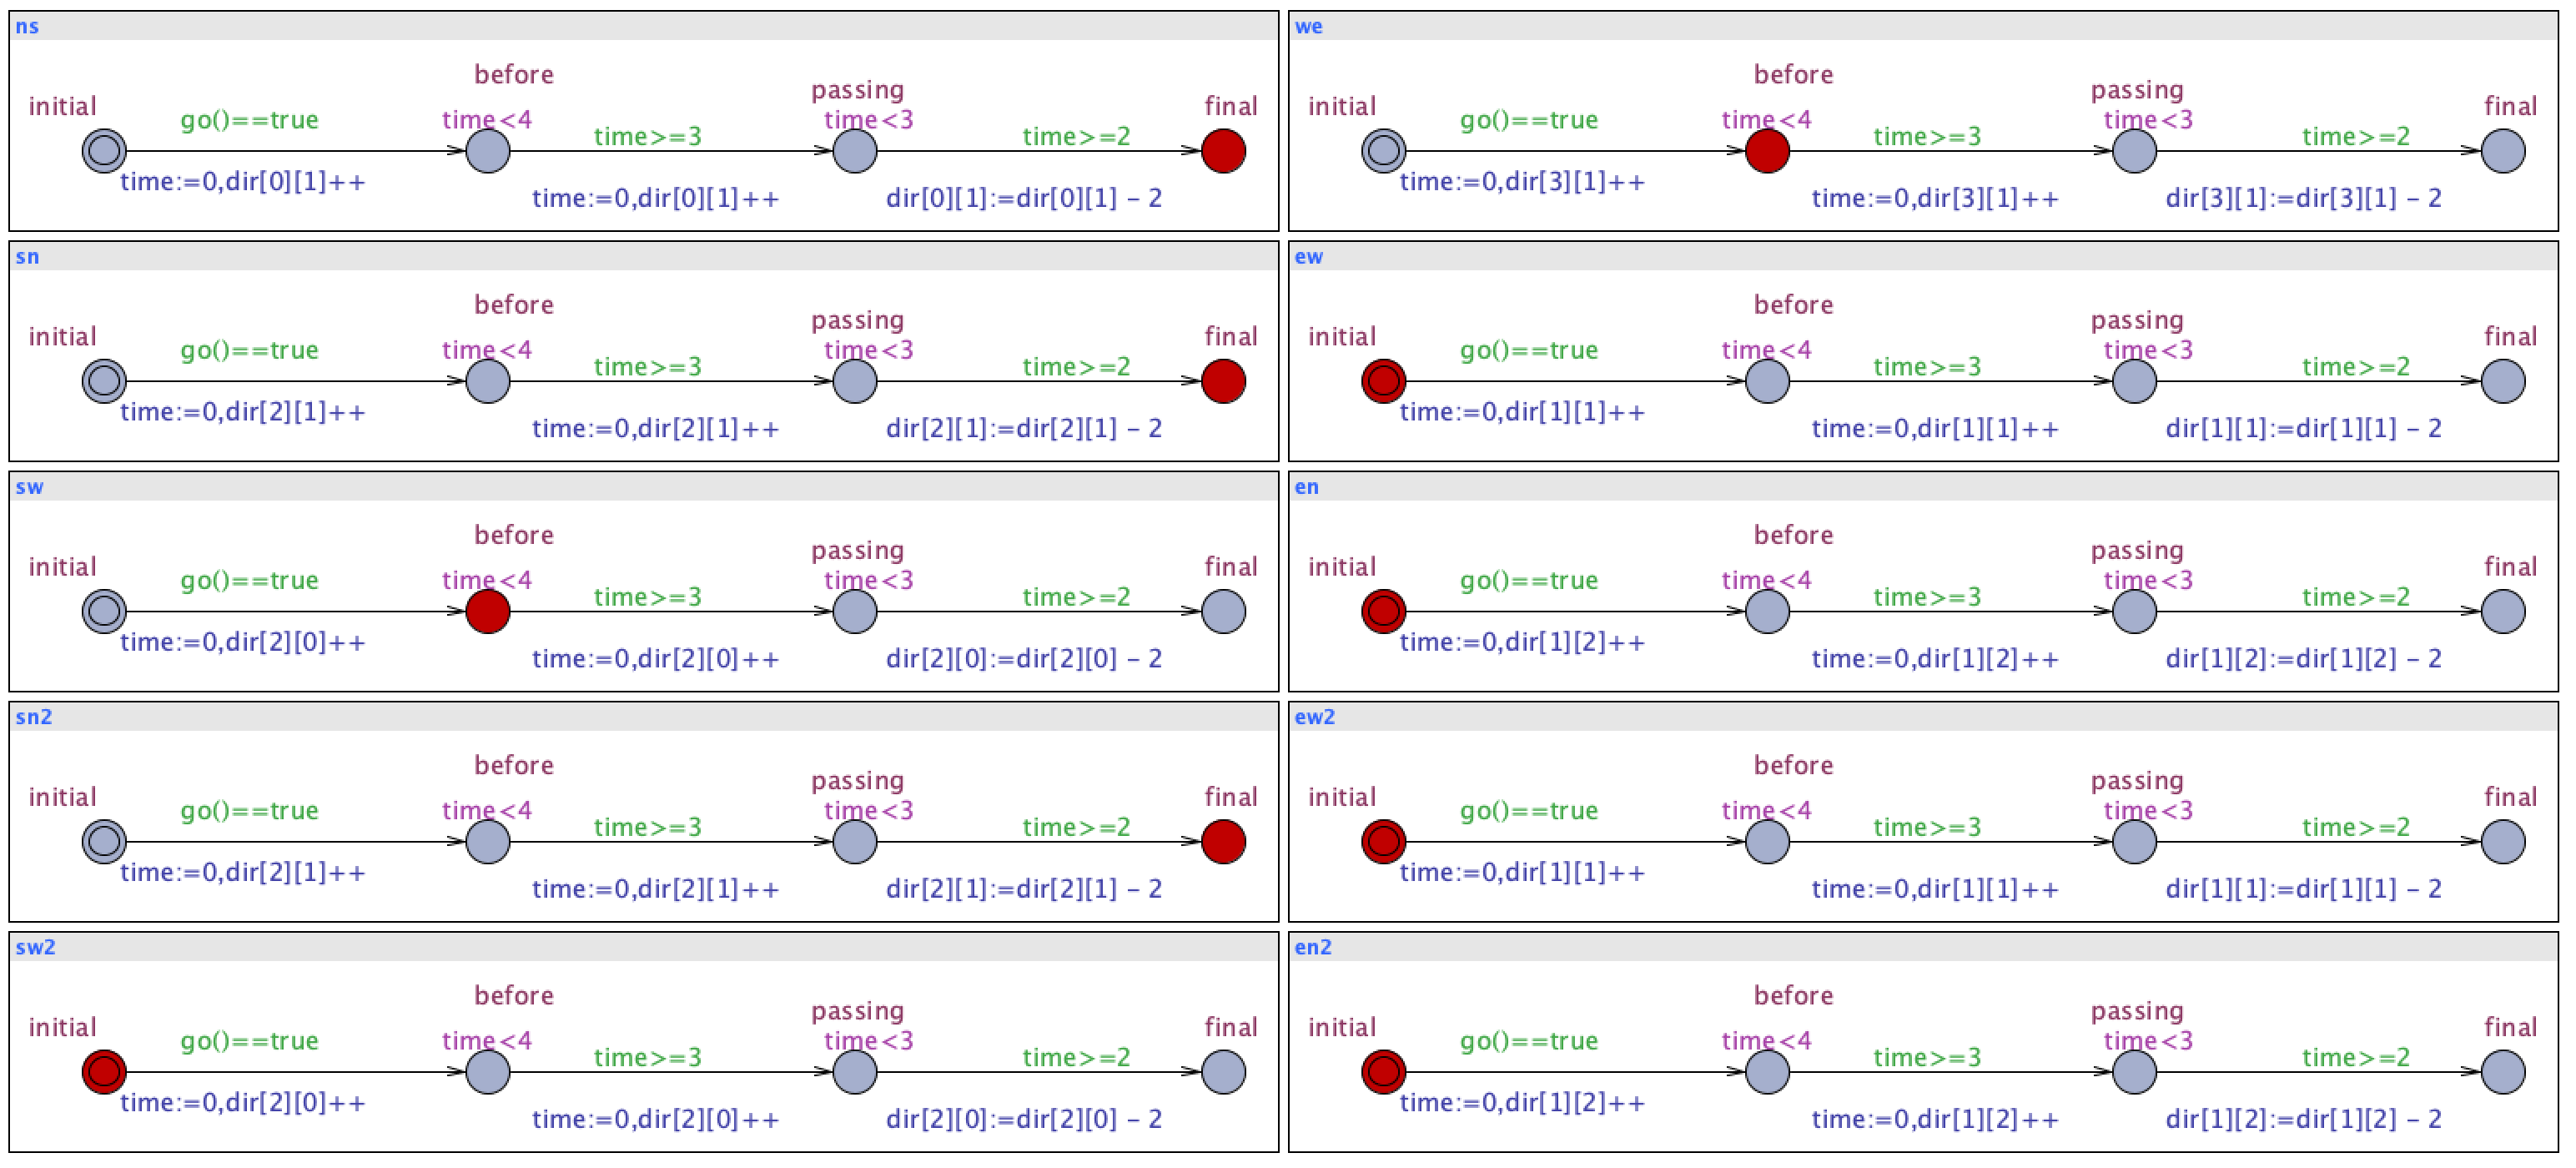
\includegraphics[width=60mm]{dArr.png}
	\caption{車両の時間オートマトンの合成}
	\label{dArr}
	\end{figure}
Fig.\ref{dArr}は10インスタンスのうち2台(we,sw)が交差点を通過前状態のスクリーンショットである.検証には大域時間変数gcを宣言する.
\subsection{モデル検査}
全ての車両インスタンスが交差点を一回通過するのにかかる最小時間について検証を行う.車両一台のinitialからfinalまでプロセスのかかる最小単位時間は5である.今回はシミュレーション時の10インスタンスで検証を行うので,例えば直進同士でまとめてを1セットとすると,2セットと右折左折のセットが2セットで合計20単位時間で通行可能ではないかと考える.試しに20単位時間で10車両が通過できるかを次の検証式を用いて検査する.
	
	\begin{verbatim}
	E<> (gc==20 and ns.final and sn.final and 
	... and en2.final)	
	\end{verbatim}
この検証式は経過時間が20単位時間の時にnsからen2までのすべての時間オートマトンが状態finalとなる実行例が存在することを示している.UPPAALモデル検査より,上記の検証式が満たされることが確かめられた.次に以下の検証式を考える.

	\begin{verbatim}
	A[] (gc<20 and ns.final and sn.final and 
	... and en2.final)	
	\end{verbatim}

この検証式は,経過時間がすべての実行例において経過時間が20単位時間未満ならばすべての時間オートマトンが状態finalにならないことを示している.UPPAALモデル検査より,上記の検証式が満たされないことが確かめられた.すなわち,より短い時間で全車両が通過する実行列が存在する.経過時間 20単位時間よりも小さい値で同様の検証を行った結果,18単位時間が最小であることが求められた.以下の 2 つの検証式が成り立つ.
	\begin{verbatim}
	E<> (gc==18 and ns.final and sn.final and 
	... and en2.final)	
	A[] (gc<18 and ns.final and sn.final and 
	... and en2.final)	
	\end{verbatim}
\section{おわりに}
本研究では,UPPAALを用いた自動運転車群制御アルゴリズムのモデル化と検証の手法を提案した.従来のものと比べ,追従を含めた本モデルでは,通過時間を短くなる通過の組み見合わせを作成可能であることを検証した.
\section*{謝辞}
本研究はJSPS科研費 JP19K11842の助成を受けたものです

\begin{thebibliography}{5}
%%%%%%%%%%%%%%%%%%%%%%%%%%%%%%%%%%%%%%%%%%%%%%%%%%%%%%%%%%%%%%%%%%%%%%%%%%%%%%%

\bibitem{u1}{Kim Guldstrand Larsen and Paul Pettersson and Wang Yi, UPPAAL in a Nutshell, International Journal of Software Tools for Technology Transfer, Vol.1, No.1-2, pp.134-152, 1997.}
\bibitem{u2}{UPPAAL, \verb$http://www.uppaal.org$}
\bibitem{u3}{Johan BengtssonWang Yi, Timed Automata: Semantics, Algorithms and Tools,  Lectures on Concurrency and Petri Nets: Advances in Petri Nets, number 3098 in LNCS, pp.87-124, 2004.}
\bibitem{a}{佐原優衣, 中村正樹, 榊原一紀, 玉置久, UPPAALを用いた自動運転車の群制御アルゴリズムの性能モデル検証, システム制御情報学会研究発表講演会(SCI'19)講演論文集, vol.63, pp.18-24,2019.}
\bibitem{a1}{M. Nakamura, Y. Sahara, C. Kojima, K. Sakakibara and H. Tamaki, Modeling and Verification of Autonomous Vehicle Group Control Algorithms, Proceedings of the SICE Annual Conference 2019 (SICE 2019), pp.115-118,2019.}
%%%%%%%%%%%%%%%%%%%%%%%%%%%%%%%%%%%%%%%%%%%%%%%%%%%%%%%%%%%%%%%%%%%%%%%%%%%%%%%
\end{thebibliography}


\end{document}
\subsection{参考文献}

文献の引用は本文中に\cite{大会ホームページ}のように書き,本文の最後に
まとめて記述します.次のフォーマットを推奨します.

\noindent
(a) 雑誌論文の場合

\noindent
番号)  著者:論文題目,雑誌名,巻(太字)-号,始ページ/終ページ(年)

\noindent
(b) 単行本の場合

\noindent
番号)  著者:書名,始ページ/終ページ,発行所(発行年)

なお,本研究が他学会で発表済みの内容の場合,その文献を参考文献に挙げるとともに,脚注で明示して下さい.

\small
